\section{Field Evidence and Engineering Discussion}
\label{sec:engineering-discussion}

\subsection{Matched Field Case at \texorpdfstring{$\varepsilon_r=4$}{eps=4}}

At $\varepsilon_r=4$,
\begin{equation}
\lambda_d=\frac{\lambda_0}{2},
\qquad
d=\lambda_0=2\lambda_d=4\frac{\lambda_d}{2}.
\end{equation}
The slab therefore contains four half wavelengths and transforms the output-air
impedance back to the input plane. The preserved field plots are evaluated at this
matched sweep value.

\begin{figure}[H]
    \centering
    \begin{subfigure}[t]{0.48\textwidth}
        \centering
        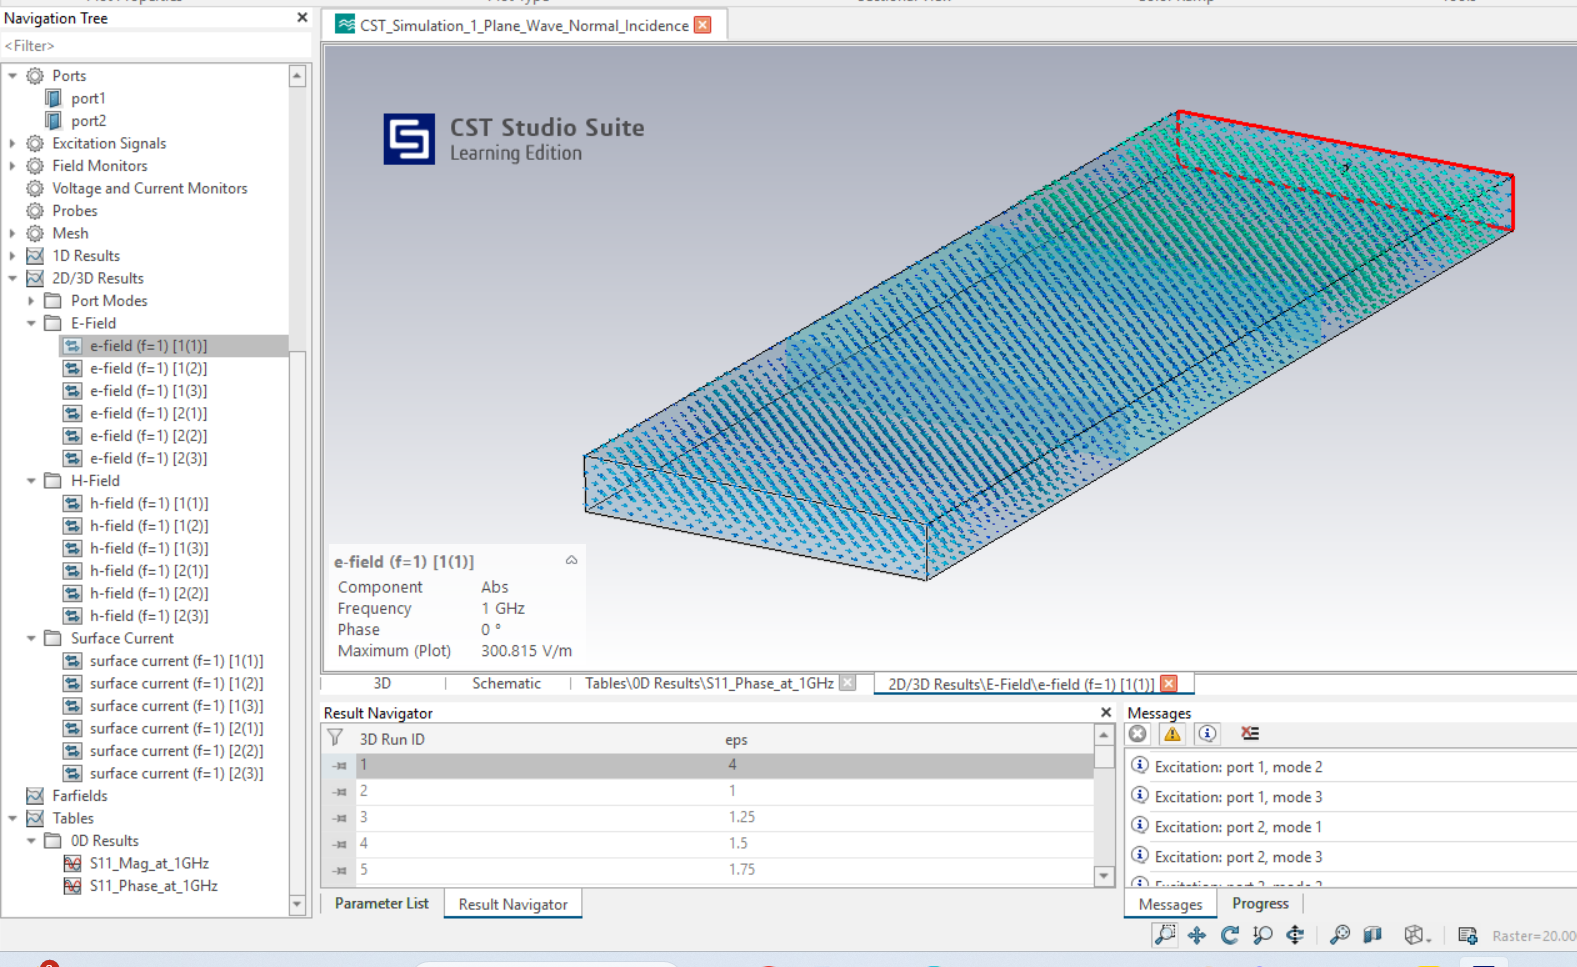
\includegraphics[width=\textwidth]{figures/cst_results/Fig_E_abs_eps4.png}
        \caption{Electric-field magnitude.}
        \label{fig:e-abs}
    \end{subfigure}
    \hfill
    \begin{subfigure}[t]{0.48\textwidth}
        \centering
        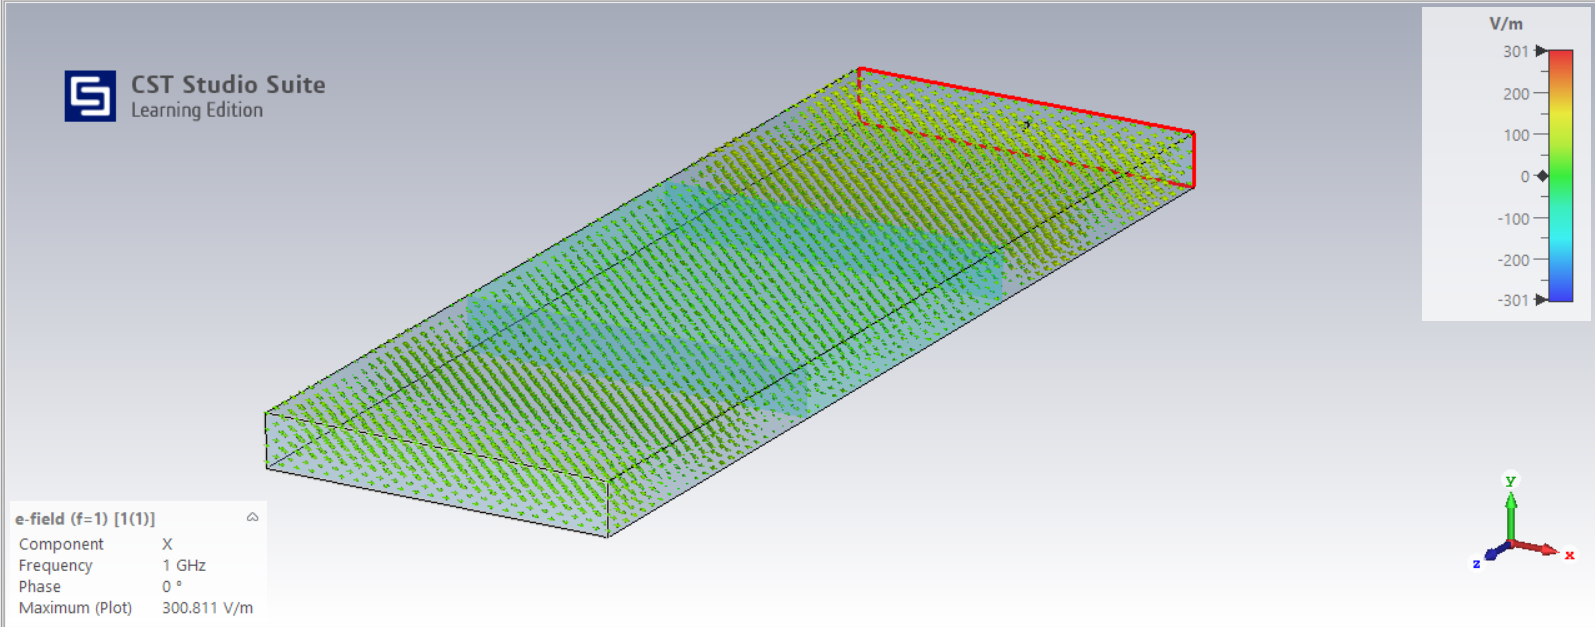
\includegraphics[width=\textwidth]{figures/cst_results/Fig_E_x_eps4.png}
        \caption{Dominant $x$-directed electric field.}
        \label{fig:e-x}
    \end{subfigure}
    \caption{Preserved electric-field evidence at 1~GHz for $\varepsilon_r=4$.}
    \label{fig:e-fields}
\end{figure}

\begin{figure}[H]
    \centering
    \begin{subfigure}[t]{0.48\textwidth}
        \centering
        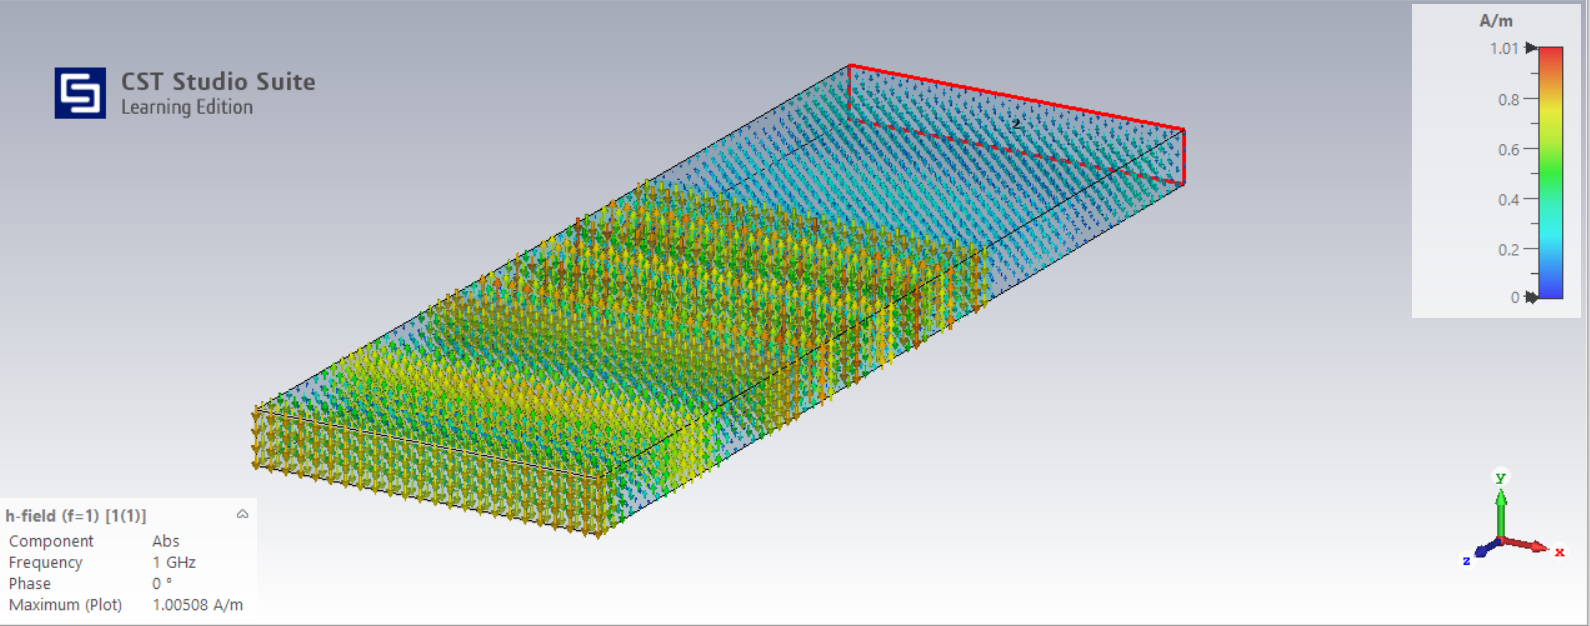
\includegraphics[width=\textwidth]{figures/cst_results/Fig_H_abs_eps4.png}
        \caption{Magnetic-field magnitude.}
        \label{fig:h-abs}
    \end{subfigure}
    \hfill
    \begin{subfigure}[t]{0.48\textwidth}
        \centering
        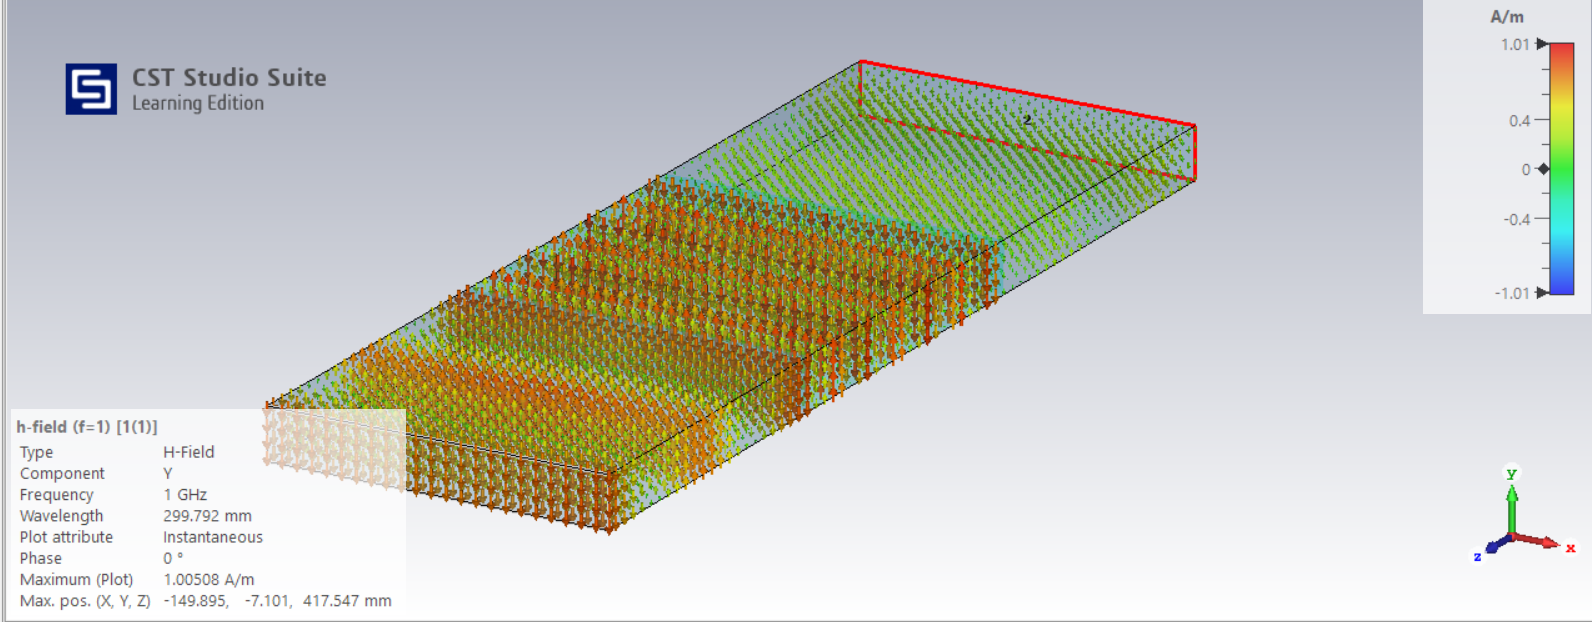
\includegraphics[width=\textwidth]{figures/cst_results/Fig_H_y_eps4.png}
        \caption{Dominant $y$-directed magnetic field.}
        \label{fig:h-y}
    \end{subfigure}
    \caption{Preserved magnetic-field evidence at 1~GHz for $\varepsilon_r=4$.}
    \label{fig:h-fields}
\end{figure}

\begin{figure}[H]
    \centering
    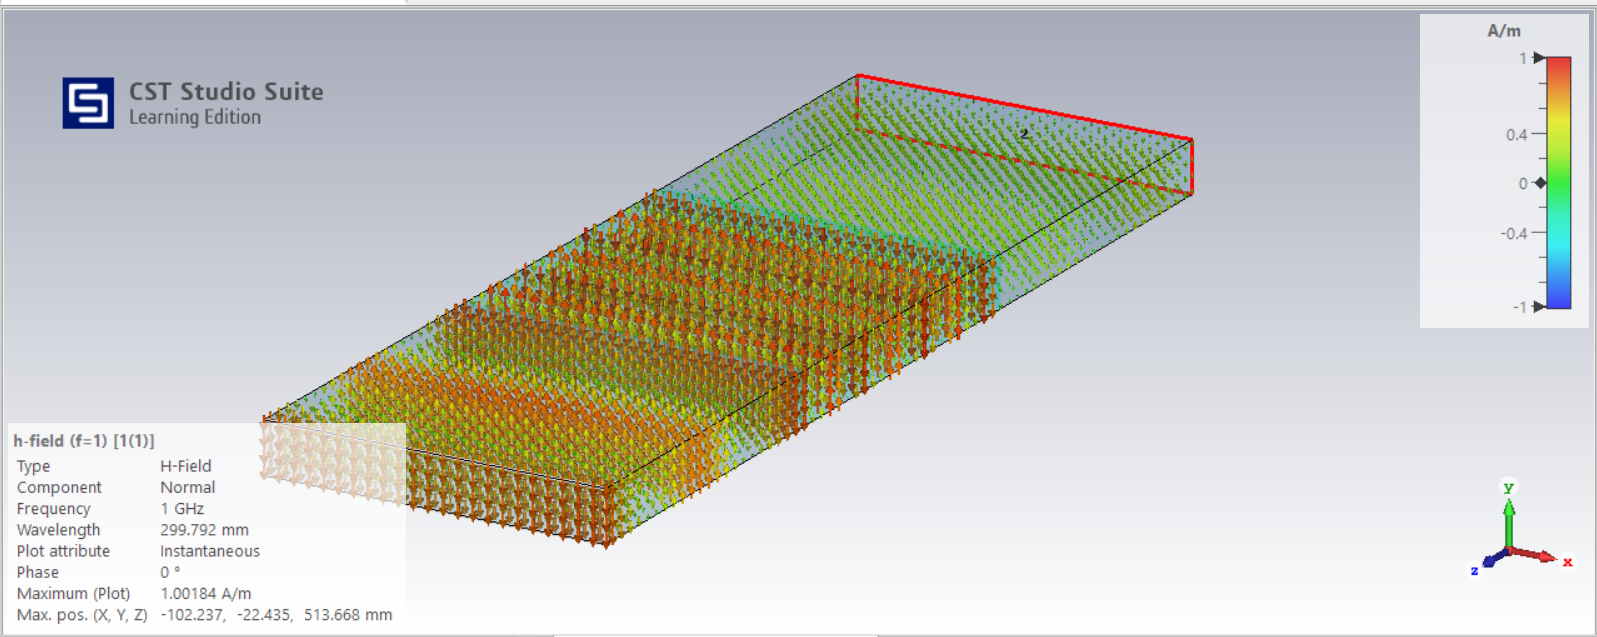
\includegraphics[width=0.82\textwidth]{figures/cst_results/Fig_H_normal_eps4.png}
    \caption{Preserved normal magnetic-field component for the selected observation
    surface at $\varepsilon_r=4$.}
    \label{fig:h-normal}
\end{figure}

The dominant transverse electric and magnetic components are consistent with the
intended TEM-like propagation environment. The screenshots are qualitative field
evidence; no raw field data or quantitative field-uniformity metric is available.

\subsection{Physical Interpretation of the Minima}

Each interface produces a partial reflection because the intrinsic impedance changes
from $\eta_0$ to $\eta_d$ and back to $\eta_0$. The input reflection is the coherent
sum of these contributions after repeated internal propagation. At an integer
half-wavelength electrical thickness, the input impedance repeats the air load, so the
net reflection approaches zero.

\subsection{Why the CST Nulls Are Nonzero}

The ideal analytical model assumes infinite transverse extent, perfect normal
incidence, an exactly lossless homogeneous slab, and exact numerical evaluation. The
preserved CST model instead uses finite transverse dimensions, waveguide ports,
finite mesh resolution, side-wall boundary approximations, and a rounded physical
length. These differences make small nonzero minima expected.

\subsection{Port-Mode Warning}

The source report records a warning that some modes at Port 2 did not reach good
accuracy and that a non-standard mode was detected. Agreement of the fundamental-mode
minimum locations with theory supports the intended physical interpretation but does
not prove that higher-order modal content is negligible. A stronger study would refine
the port mesh, vary the number of requested modes, inspect modal fields and cutoff
behavior, and demonstrate convergence of $S_{1(1),1(1)}$.

\subsection{Numerical Reliability}

No mesh-convergence, boundary-size sensitivity, port-length sensitivity, or raw-data
comparison is preserved. Consequently, the report treats the minimum locations as
validated qualitative and discrete quantitative evidence, while treating the exact
null depths as fixed-model outputs rather than convergence-qualified predictions.
